% Template for ISBI-2017 paper; to be used with:
%          spconf.sty  - ICASSP/ICIP LaTeX style file, and
%          IEEEbib.bst - IEEE bibliography style file.
% --------------------------------------------------------------------------
\documentclass{article}
\usepackage{spconf,amsmath,graphicx}
\usepackage{epstopdf}
\usepackage{amsmath}
\usepackage{xcolor}
\usepackage{algorithm}
\usepackage{subfig}
\usepackage{algorithmic}        %用到的宏包,要自己改下

\usepackage{multirow}
\usepackage{tikz}
\renewcommand{\algorithmicrequire}{\textbf{Input:}}   %改成后面的小标题

\renewcommand{\algorithmicensure}{\textbf{Output:}}
% --------------------
\def\x{{\mathbf x}}
\def\L{{\cal L}}

% Title.
% ------
\title{ Faster Background Removal in 3D Fluorescence Microscopy Images Using Multi-Channel Information}
%
% Single address.
% ---------------
\name{Author(s) Name(s)\thanks{Thanks to XYZ agency for funding.}}
\address{Author Affiliation(s)}
%
% For example:
% ------------
%\address{School\\
%	Department\\
%	Address}
%
% Two addresses (uncomment and modify for two-address case).
% ----------------------------------------------------------
%\twoauthors
%  {A. Author-one, B. Author-two\sthanks{Thanks to XYZ agency for funding.}}
%	{School A-B\\
%	Department A-B\\
%	Address A-B}
%  {C. Author-three, D. Author-four\sthanks{The fourth author performed the work
%	while at ...}}
%	{School C-D\\
%	Department C-D\\
%	Address C-D}
%
% More than two addresses
% -----------------------
% \name{Author Name$^{\star \dagger}$ \qquad Author Name$^{\star}$ \qquad Author Name$^{\dagger}$}
%
% \address{$^{\star}$ Affiliation Number One \\
%     $^{\dagger}$}Affiliation Number Two
%
\begin{document}
%\ninept
%
\maketitle
%
\begin{abstract}
Background noise remains a significant problem in the 3D fluorescence microscopy images. On the one hand, the model of background noise used widely isn't accurate, on the other hand, we need a fast algorithm to estimate the background noise for the large sizes of 3D image data(over $10^{11}$ voxels). In this paper, we present a new algorithm to estimate background noise assisted by the multichannel information\\
\end{abstract}
%
\begin{keywords}
fluorescence microscopy image, haze, multichannel, background removal
\end{keywords}
%
\section{Introduction}
\label{sec:intro}
 In thise paper, we present a faster background removal algorithm than [1]  with the help of multi-channel information that is capable of precisely identifying and removing background noise in such large volume 3D images.\\
	There have been a lot of methods for removing background noise in microscopy images, such as spatial filtering, rolling ball algorithms, fitting smoothly varying function, entropy minimization, and matrix rank minimization. However, due to the rapidly increasing sizes of image data, the time and space complexities of some sophisticated methods(e.g, optimization based methods and function fitting methods) are too high. With whole-body imaging fields yield not only large data size but also wide variations in the sizes of foreground objects. Although simple methods like spaltial filtering and rolling ball algorithms are quite fast, significant variance of foreground objects can greatly affect their performance. For example, in some parts of our brain tumor images, cells are uniformly distributed, for which small window/ball sizes give the best performance; in other parts, tumor cells are clustered closely together and form much larger target objects, for which small window/ball sizes may include tumor cell clusters as part of the background(to be removed). We call those "small" windows that cause removal of foreground objects the undersized windows.\\
	\\
	In [1], it develops a background removal algorithm based on spatial filtering algorithm. Their motivation is to overcome "undersizede window" issue in spatial filtering. The steps of  spatial filtering are as follow:
	\begin{enumerate}
		\item Choose a fix window size to slip the whole images.
		\item Set the thresholds for each window to seperate foreground signals and background noises.
	\end{enumerate}
	Some windows may be filled with all foreground signals, others may be fill with background noises.
	For the shape of tissue in each windows are different, so if we choose one threshold for all windows, the results of background removal sometimes are poor. Therefore, [1] proposed the "undersized window" issue. They choose a fixed threshold for all windows at first and get the intensity of thresholds in each windows. Then they use one-class learning method to detect the "undersized windows" which can be considered as outliers. These outliers comes from "undersized windows".
	[1] improves the results of spatials filtering like rolling ball indeed, but the running time of one-class learning are still huge. It will takes a whole day for a 1024*1024*85 stack images. So we present a new algorithm to estimate the background noise with the help of multichannel information intead of one-class learning. The time complexity of our algorithm is O(n) that speeds up a lot.
\section{Method}
\label{sec:format}
Firstly, we use our new algorithm to estimate the background noise. Secondly, we use our new model the recover the real images.
\subsection{Estimate Background Noise}
First, we assume that:
\begin{itemize}
	\item The images of one tissue from any two channels are not overlapped.
	\item The intensity of signals in one channel must be larger than the intensity of background noise in other channels.
\end{itemize}
We always compare the images from two channels in the same depth. Because images from different channels are independent, we need nomalize them at first if we want to compare them. When multichannel microscopy images satisfied the above assumptions, if the intensity values of pixels in one channels are smaller than the maximum value of pixels in the other channels, then we can consider this pixels must be background noise and the intensity of this pixel is the intensity of background. Because background noise variou slowly, the background noise of the whole images in this depth can be computed by linear interpolation based on these pixels which must be background. Our method avoids the "undersized windows" issue, so we needn't one-class learning to detect undersizes window. For example, we have two channel images, such as Figure \ref{fig:actin_44} (a) and (b). Because one-class learning costs the most of time in [1], so our algorithm is much faster than [1].   \\
\begin{figure}
\subfloat[actin]{
	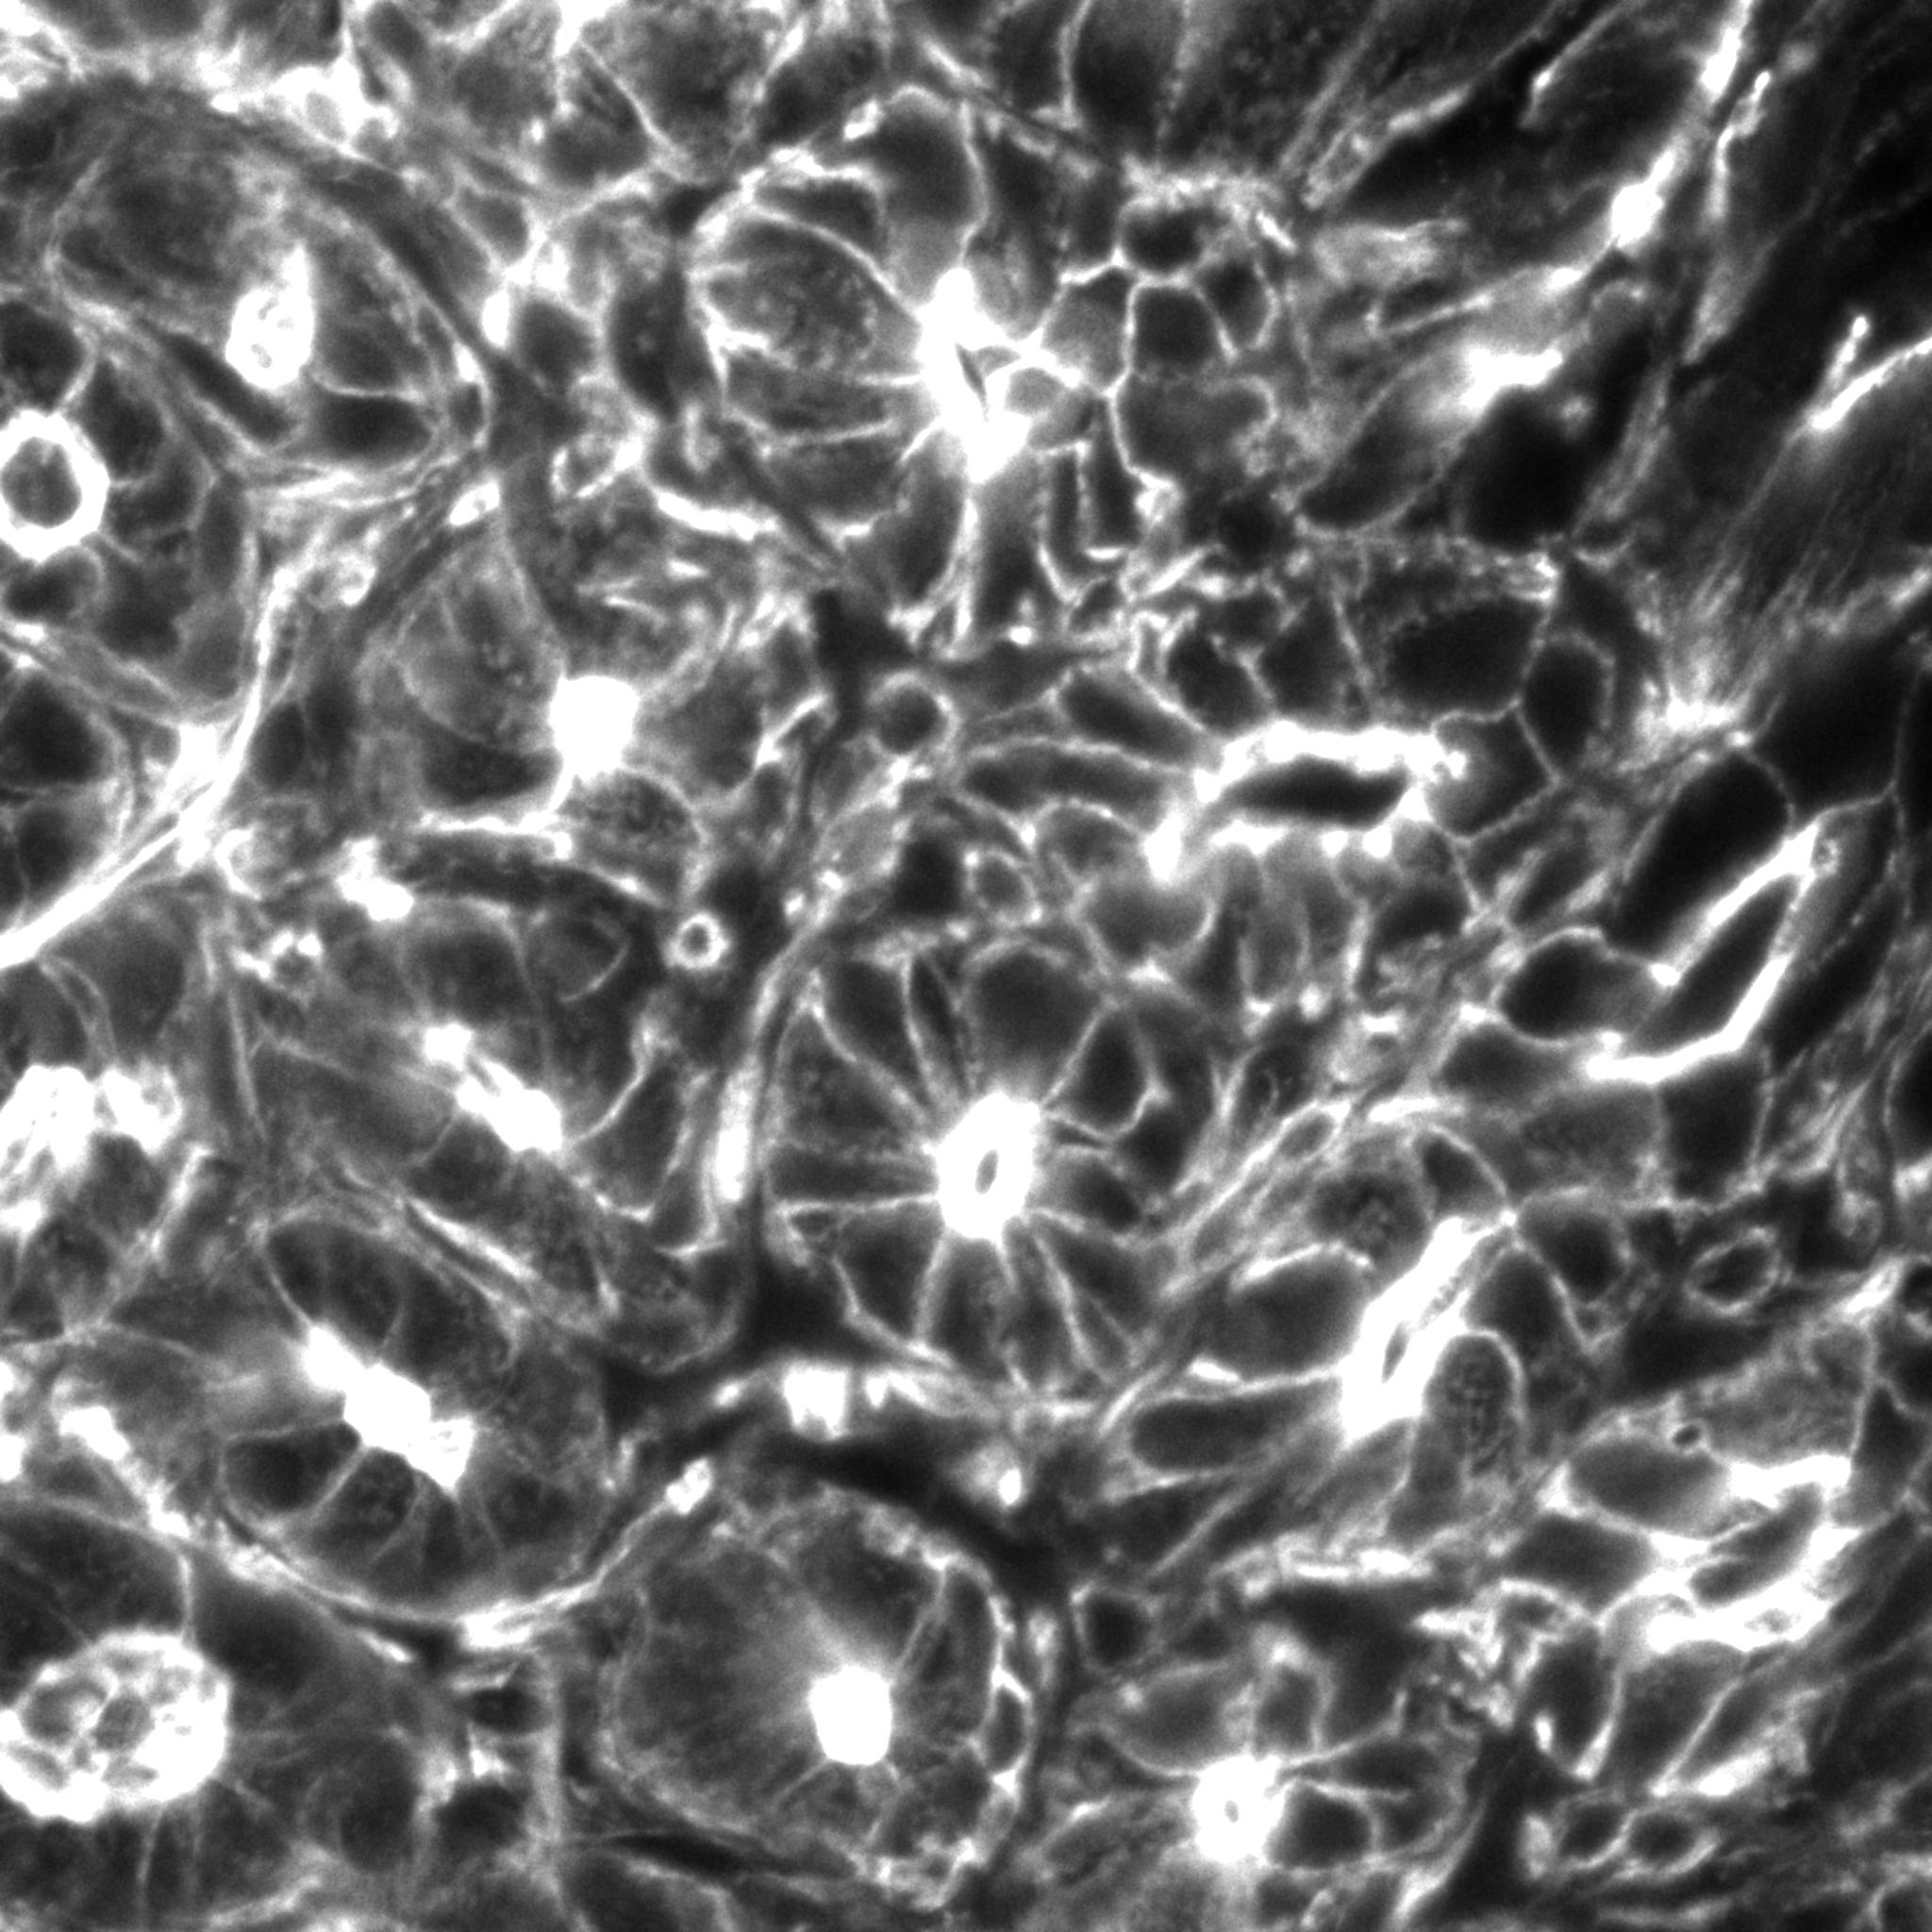
\includegraphics[width=0.25\textwidth]{8bits_3D_Mean_actin_44.png}
}
\subfloat[nucleus]{
	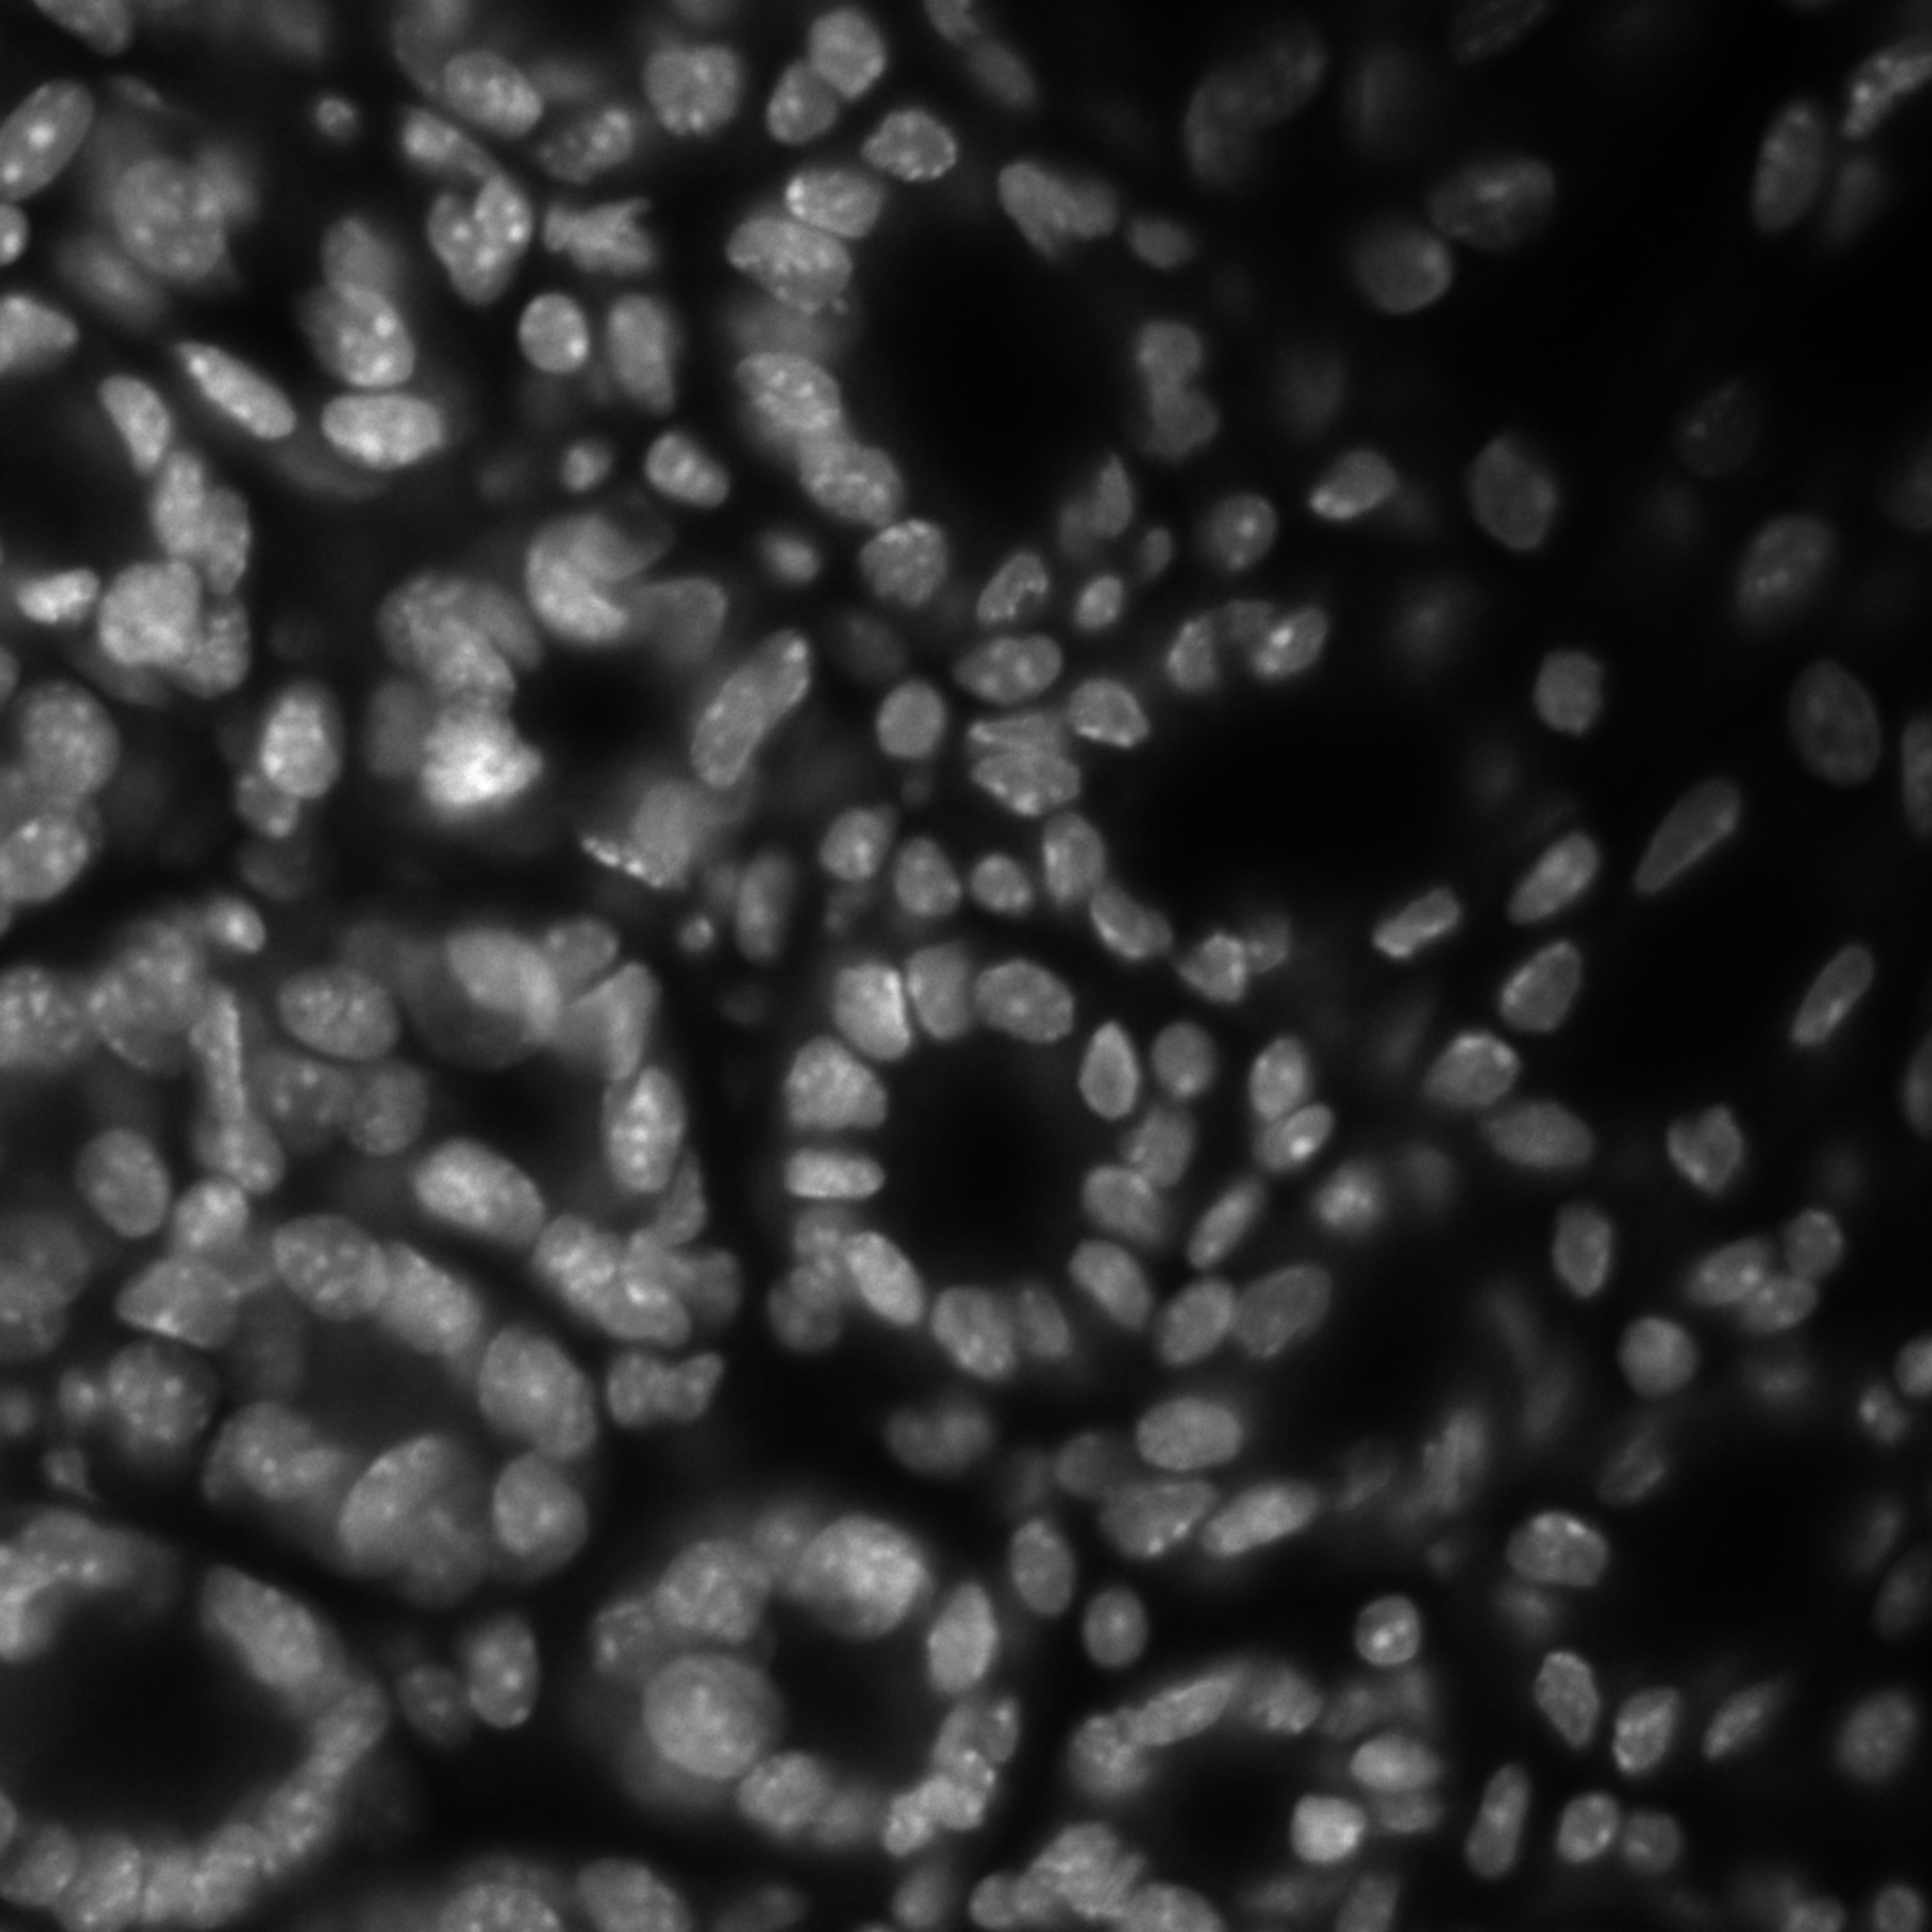
\includegraphics[width=0.25\textwidth]{8bits_3D_Mean_nucleus_44.png}
}

\subfloat[background generated by (a) subtract (b)]{
	\includegraphics[width=0.25\textwidth]{background_440001.png}
}
\subfloat[background of whole image]{
	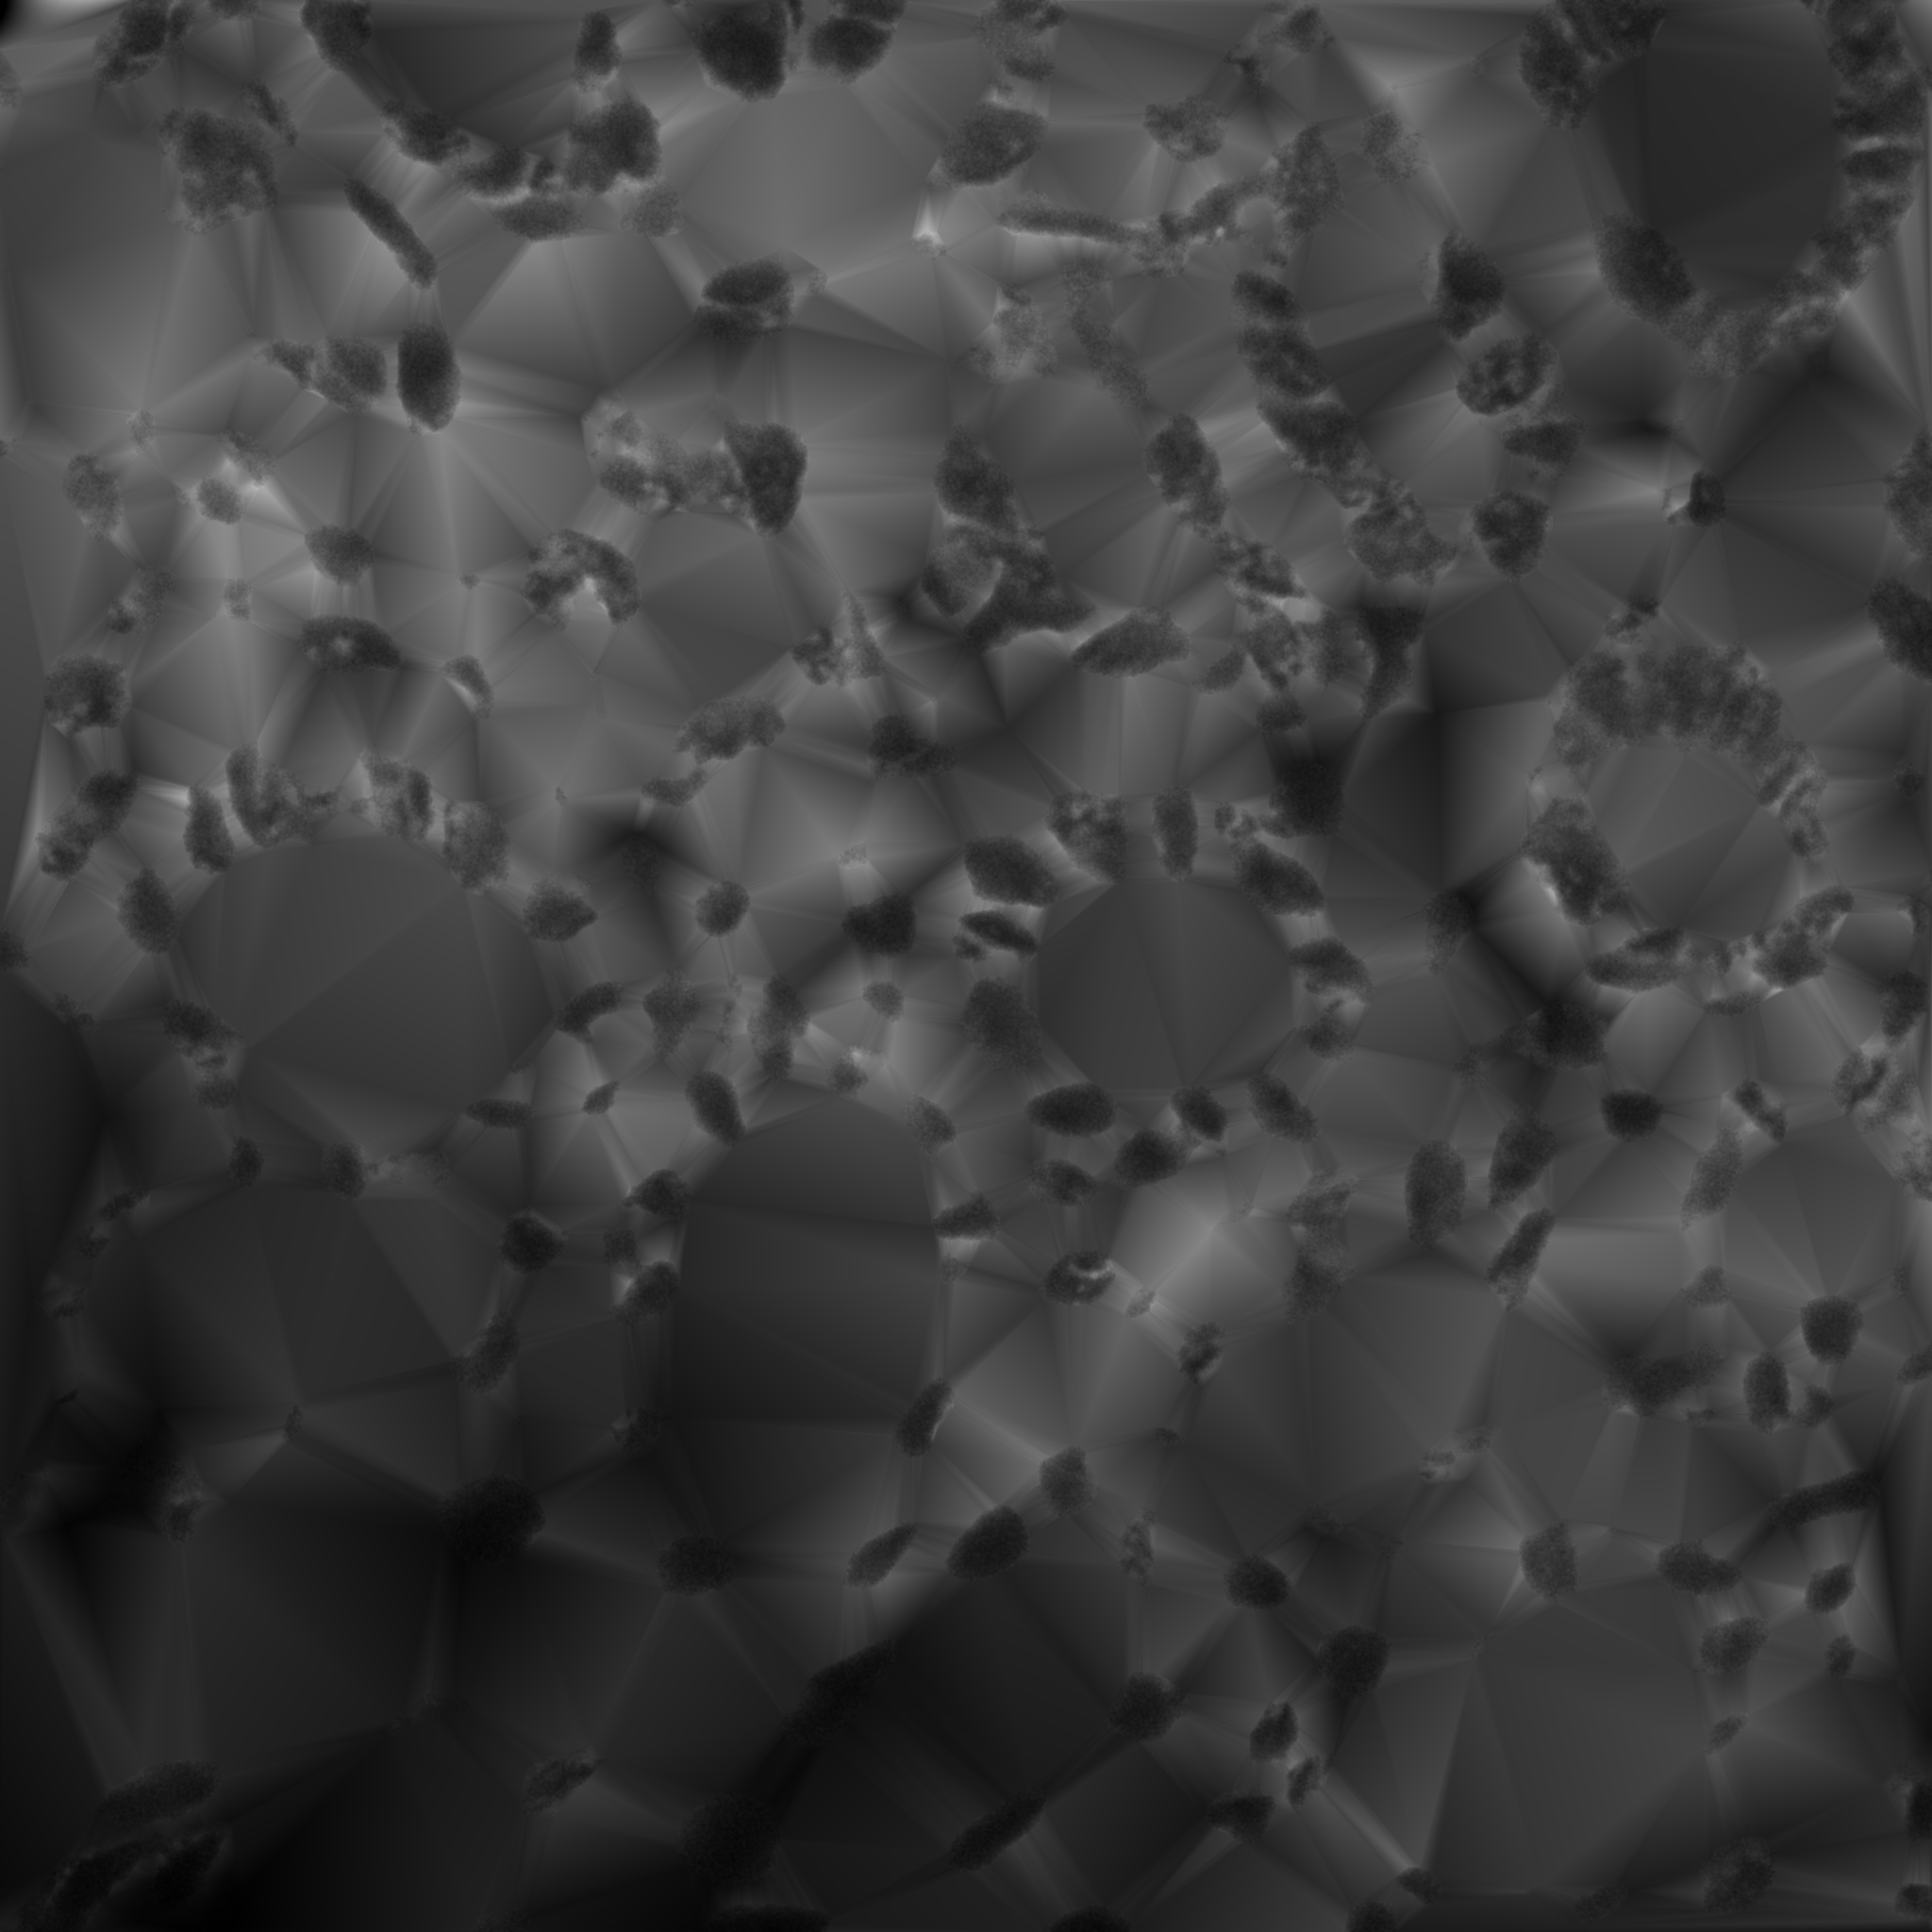
\includegraphics[width=0.25\textwidth]{8bits_actin_background_scatter.png}
}

\subfloat[]{
	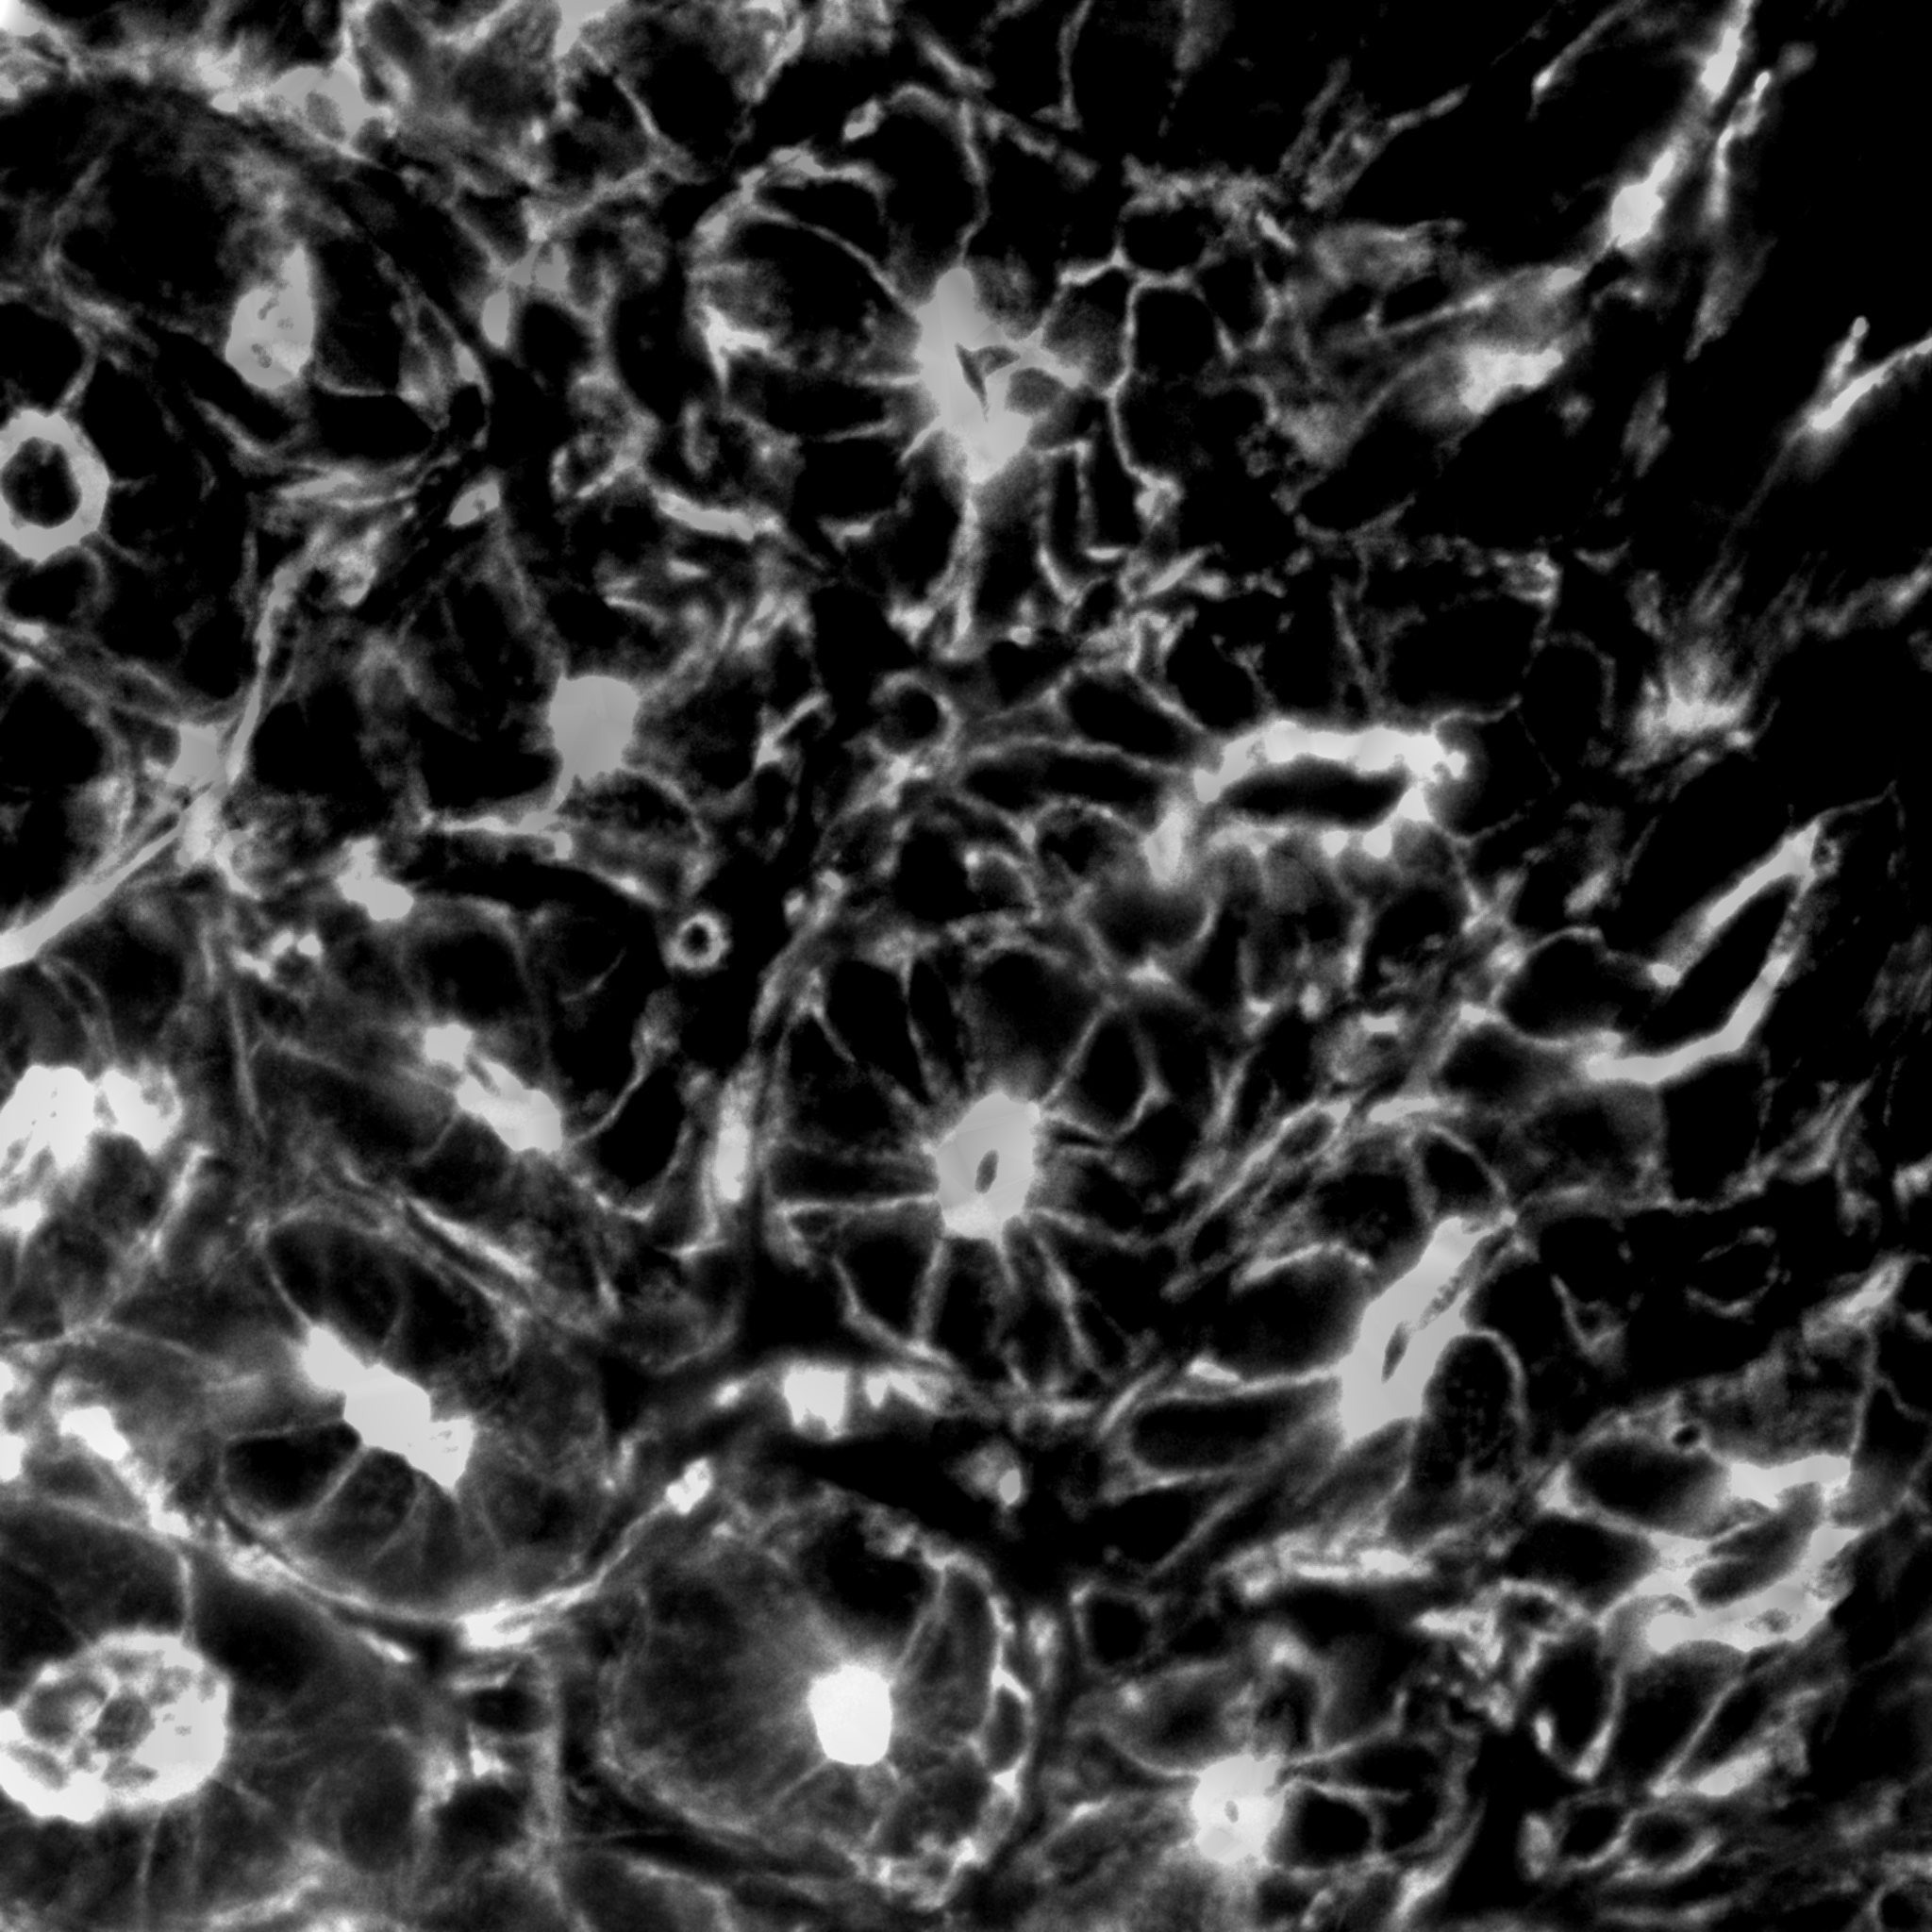
\includegraphics[width=0.25\textwidth]{8bits_actin_new_image.png}
}
	\caption{(a) and (b) are actin and nucleus respectively. They are two channels of one tissue. (c) is the background generate by the first step of our algorithm. We use substract (a) from (b), then the intensity of area whose pixels are smaller than zero is (c). (d) is the estimated background noise of whole images generated by linear interpolation using (c). (e) is our result generated by subtract (a) from (d).}
	\label{fig:actin_44}
\end{figure}

\begin{algorithm}[htb]    %算法的开始
	\caption{Background Removal based on Multichannel Images}   %算法的标题
	\label{alg:Framwork}       %给算法一个标签,这样方便在文中对算法的引用
	\begin{algorithmic}[1]     %这个1 表示每一行都显示数字
		\REQUIRE ~~ $C_1$, $C_2$,...$C_n$\\
		\STATE Normalization($C_1$,...,$C_n$)                          %算法的输入参数:Initialization
		\FOR{$k = 1$ to $n$}
			$NC_k$ = $C_k$ - $\max\limits_{1 \leq j \leq n, j\neq i}$ C_j
		\ENDFOR
		\FOR{$k = 1$ to $n$}
			\FOR{$p \in NC_i$}
				\IF{$p == 0$}
					$B_k(coordinate(p)) = C_k(coordinate(p))$
				\ELSE
					$B_k(coordinate(p)) = -1$
				\ENDIF
			\ENDFOR
		\ENDFOR
		\FOR{$k = 1$ to $n$}
			$B_k$ = interpolation($p \in B_k $ if p \neq -1)
		\ENDFOR
		\ENSURE ~~ $B_1$, $B_2$,...$B_n$\\                           %算法的迭代:Iteration
		\end{algorithmic}
	\end{algorithm}
If the two above assumptions are always right, our algorithm is always right undoubtedly. However, they are not satisfied in some extreme suitations.\\
For assumption 1, ....\\
For assumption 2, the intensity of foreground signals decreses from the position of real signals gradully, not immediately like Figure \ref{fig:single}. So if two signals are two close, we will get the images like Figure \ref{fig:two_points}. This case dissatisfy the assumption 2, but we can set the threshold of the maximal value of the background noise to avoid making mistakes. It means that we can't consider these pixels are background even if they are smaller than zero when has been subtracted by the maximal value of other channels if their original intensity are larger than the threshold.
\begin{figure}
	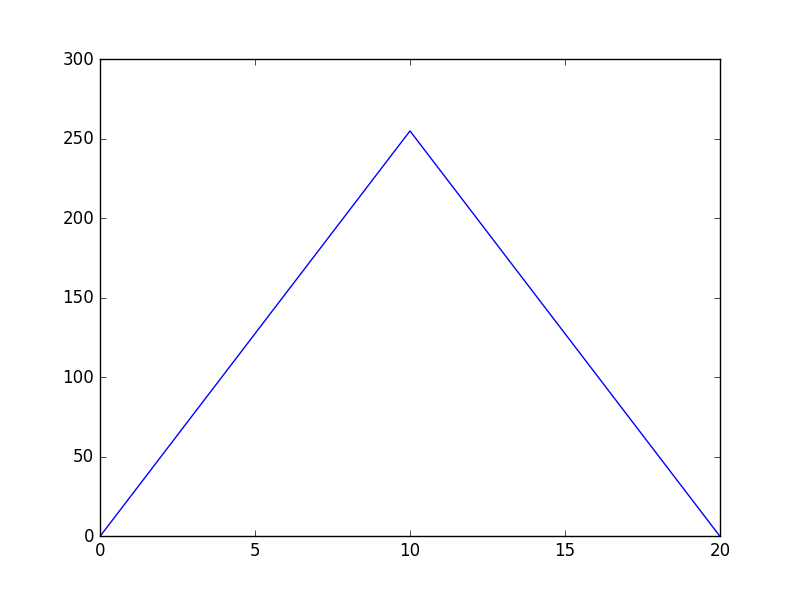
\includegraphics[width=0.5\textwidth]{figure_1.png}
	\caption{We draw a segement in one image, then we can get the garph of intensities in this line. X-axis represents the coordinate in this line, while Y-axis represents the intensity of corresponding pixels. In fact, there is only real signal when x = 10, but we will get this picture in the end.}
	\label{fig:single}
\end{figure}

\begin{figure}
	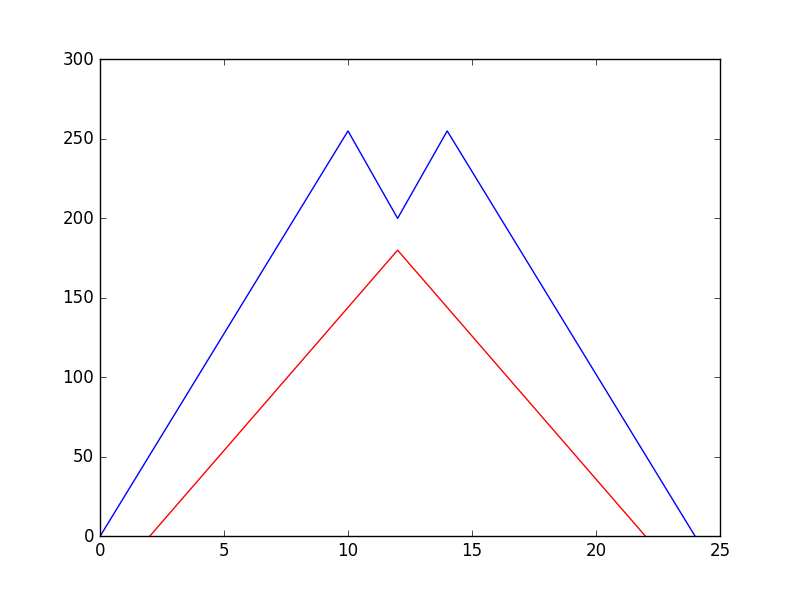
\includegraphics[width=0.5\textwidth]{figure_2.png}
	\caption{The signals of blue line and the ones of red lines are from different channels. According to the model we describe in Figure \ref{fig:single}, the peak of the red lines should be foreground singal, and the blue point above the peak should be background noise.}
	\label{fig:two_points}
\end{figure}
\subsection{Recover the Real Image}
We think the $$I = Jt + B$$, where I is intensity, J is the real image, t is reflectivity ratio, B is the background.






% To start a new column (but not a new page) and help balance the last-page
% column length use \vfill\pagebreak.
% -------------------------------------------------------------------------
\vfill
\pagebreak


\section{REFERENCES}
\label{sec:ref}

List and number all bibliographical references at the end of the paper.  The references can be numbered in alphabetic order or in order of appearance in the document.  When referring to them in the text, type the corresponding reference number in square brackets as shown at the end of this sentence \cite{C2}.

% References should be produced using the bibtex program from suitable
% BiBTeX files (here: strings, refs, manuals). The IEEEbib.bst bibliography
% style file from IEEE produces unsorted bibliography list.
% -------------------------------------------------------------------------
\bibliographystyle{IEEEbib}
\bibliography{strings,refs}

\end{document}
